%% F2
\begin{figure*}[ht]
  \begin{subfigure}{.315\textwidth}
    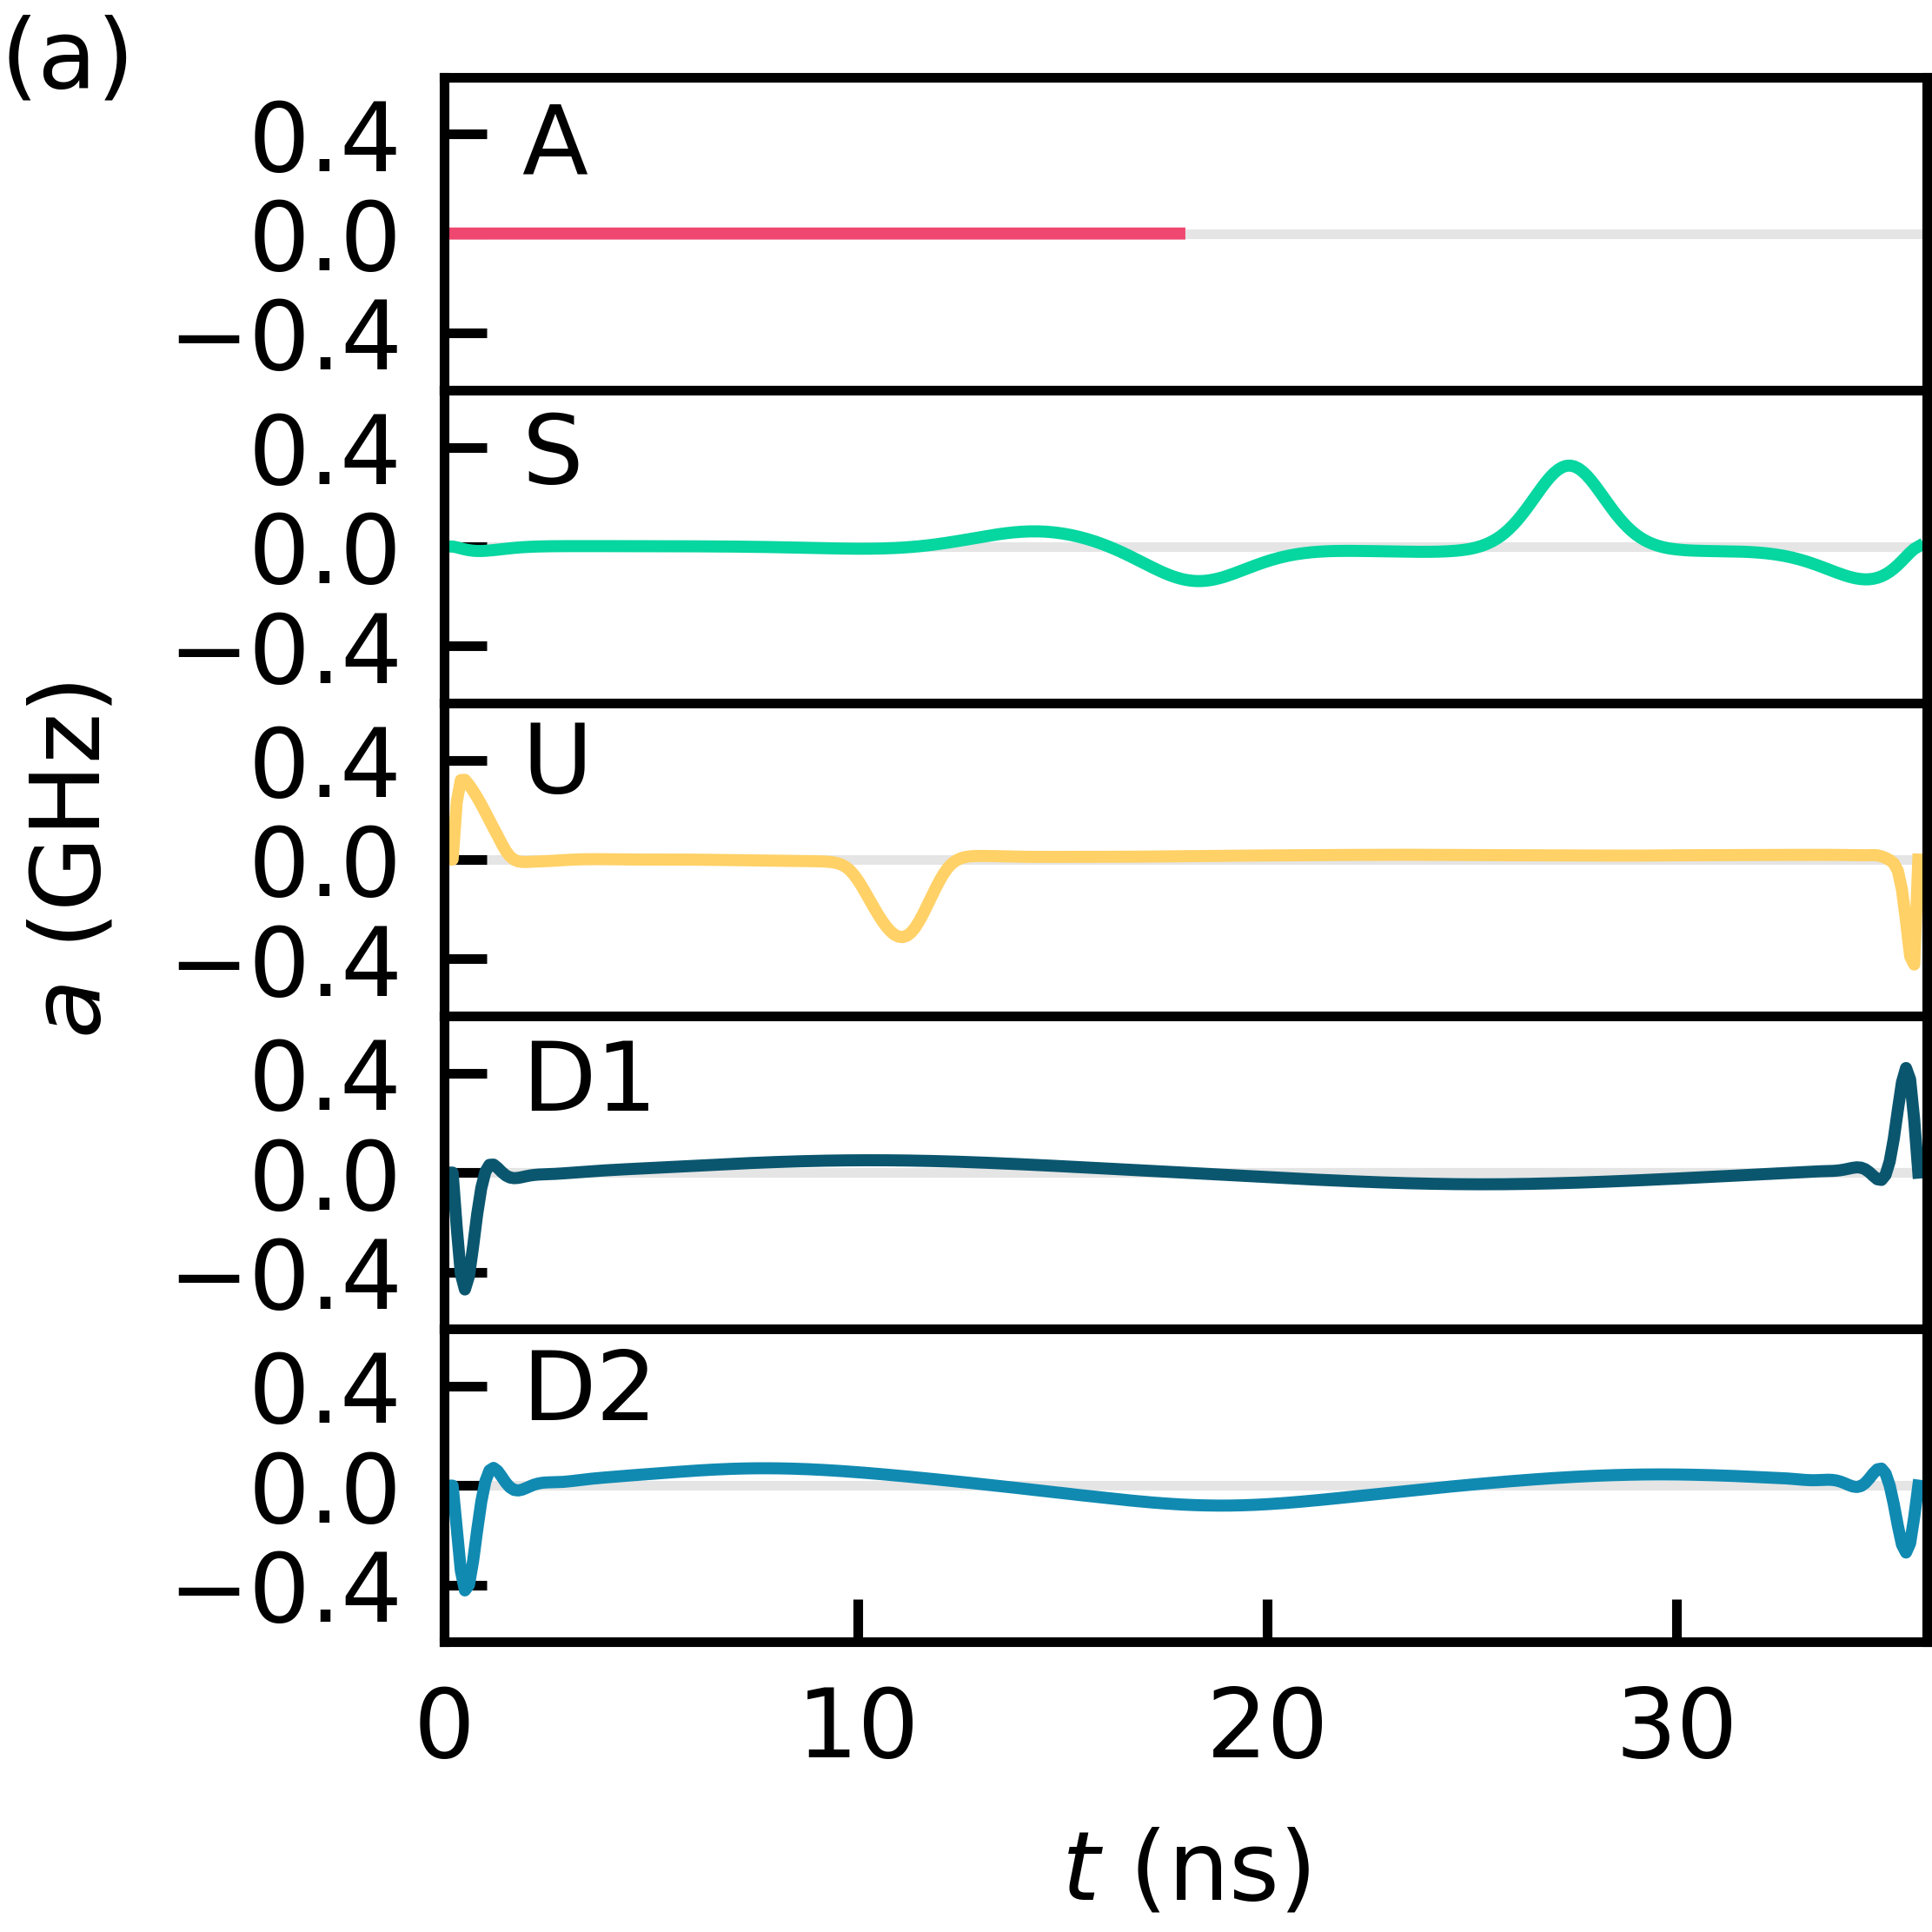
\includegraphics[width=\linewidth]{assets/f2a.png}
    \caption{\label{fig:statica}}
  \end{subfigure}\hfill
  \begin{subfigure}{.4\textwidth}
    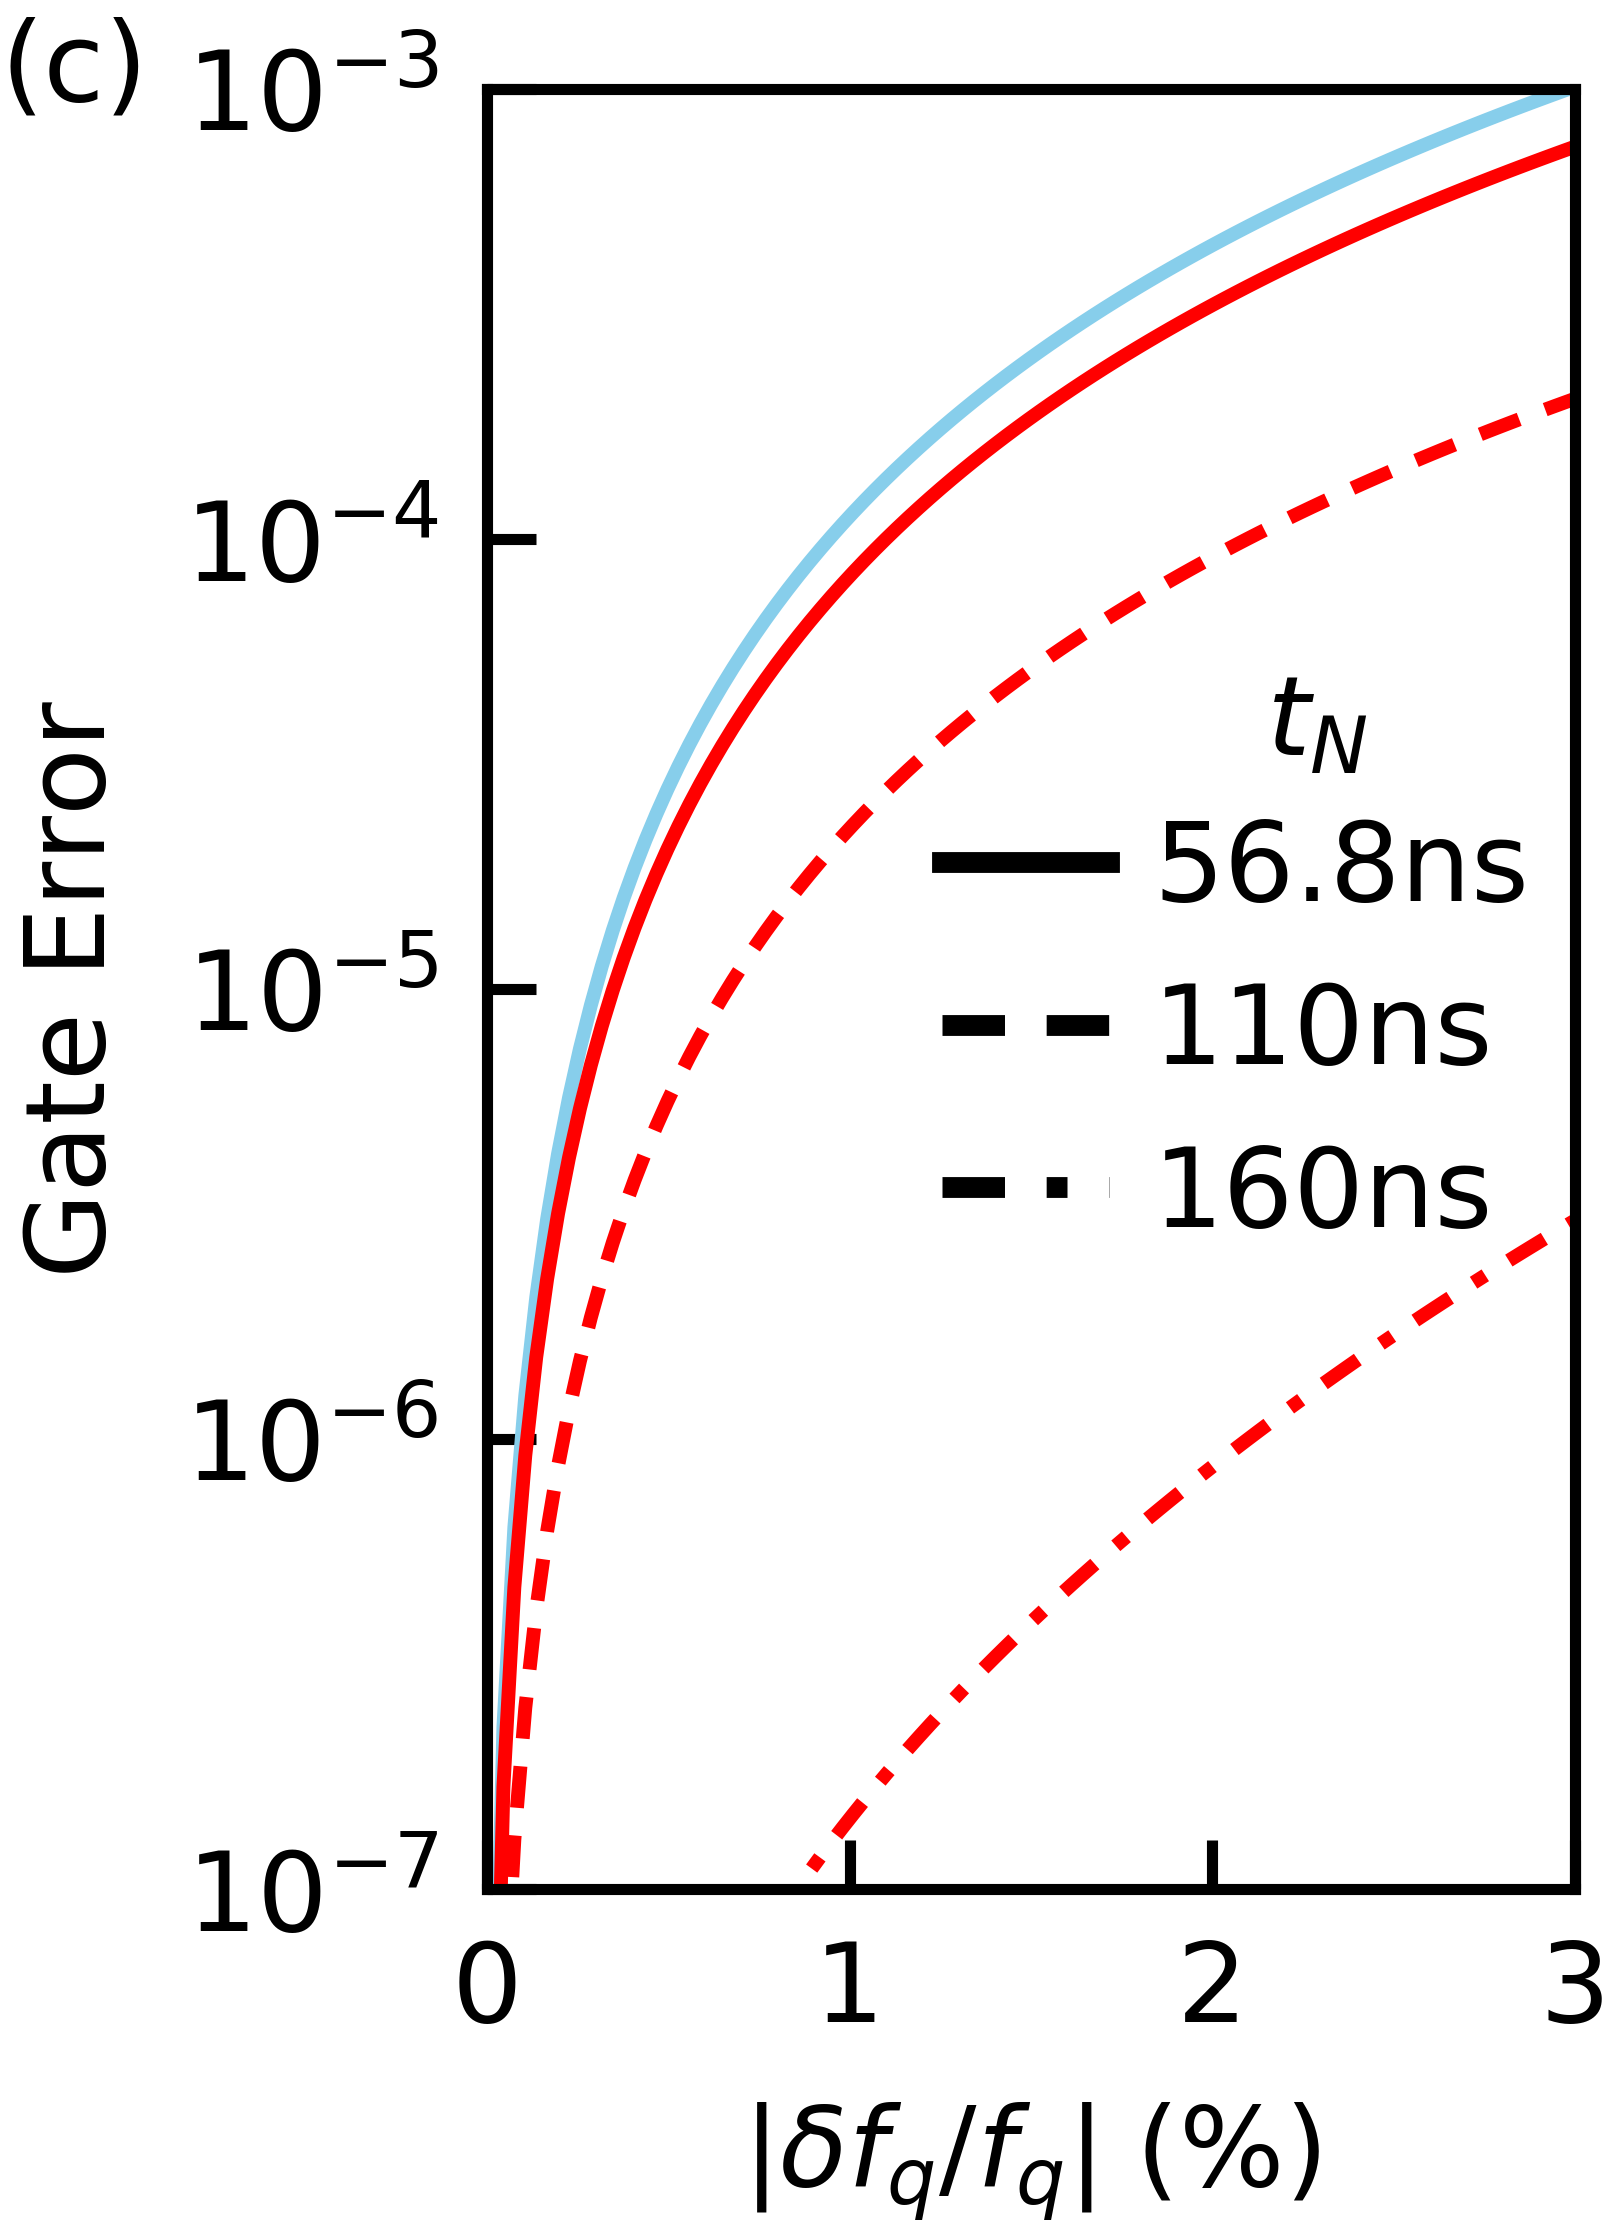
\includegraphics[width=\linewidth]{assets/f2b.png}
    \caption{\label{fig:staticb}}
  \end{subfigure}\hfill
  \begin{subfigure}{.23\textwidth}
    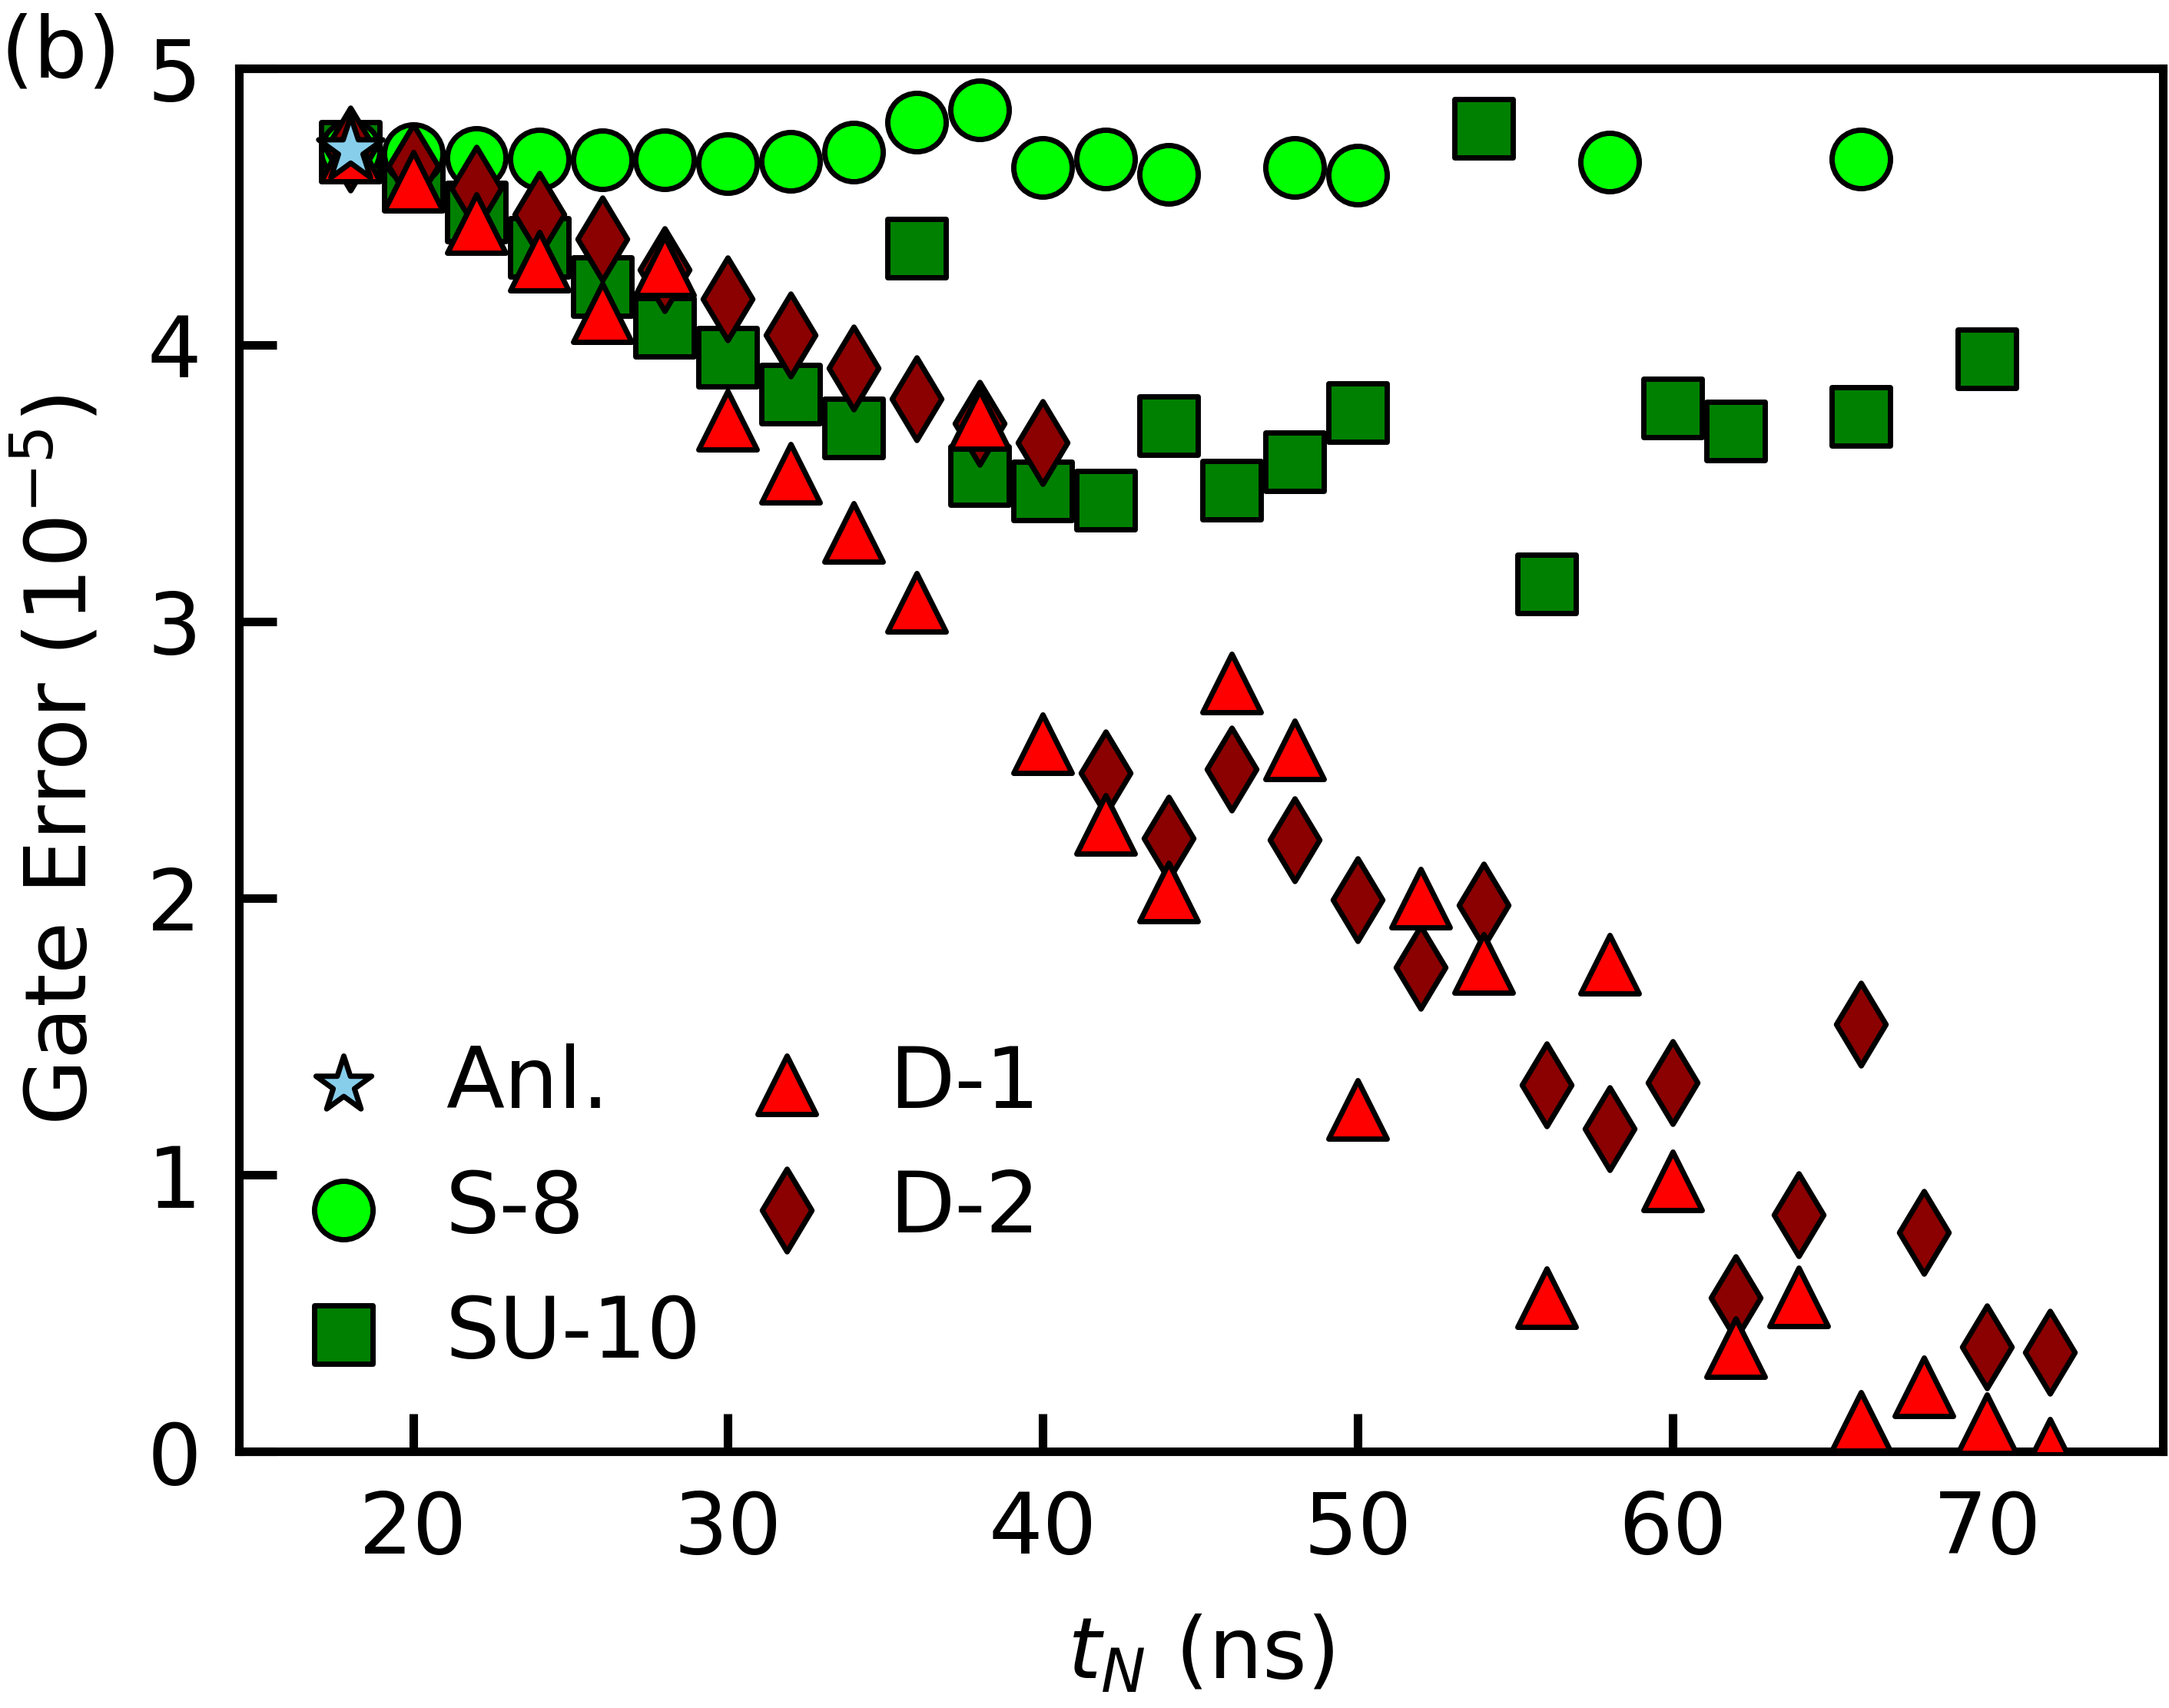
\includegraphics[width=\linewidth]{assets/f2c.png}
    \caption{\label{fig:staticc}}
  \end{subfigure}
  \caption{
    (a) Flux pulses for $Z/2$ gates robust to qubit frequency detunings constructed with the
    analytic (A), sampling (S), unscented sampling (U), and the 1\textsuperscript{st}-
    and 2\textsuperscript{nd}-order derivative methods (D1, D2). The flux pulses shown
    for the sampling, unscented sampling, and derivative methods are optimized
    for twice the gate time of the analytic gate.
    (b) Single gate error at a one-percent qubit frequency detuning as
    a function of the gate time. Missing
    data points represent gates with a gate error greater than $5 \cdot 10^{-5}$.
    (c) Single gate error as a function of the qubit frequency detuning.
    The gate errors for the analytic and 1\textsuperscript{st}-order derivative
    methods are shown for gate times which are multiples of $1 / 4 f_{q} \sim 18 \textrm{ns}$.
    The gate errors for the two methods are
    indistinguishable at the gate time $18 \textrm{ns}$.
  }
  \label{fig:static}
\end{figure*}

\section{Robustness to Static Parameter Uncertainty \label{sec:static}}
We have formulated the QOC
problem as an open-loop optimization problem; equivalently,
we do not incorporate feedback from the experiment in optimization.
However, the device's parameters deviate from the parameters we use in optimization,
leading to poor experimental performance. We combat errors
of this form using robust control techniques,
making the state evolution insensitive
to parameter uncertainty. As an example,
we mitigate errors arising from the drift and finite measurement
precision of the qubit frequency, which modifies the fluxonium Hamiltonian
\eqref{eq:hamiltonian} by $f_{q} \rightarrow f_{q} + \delta f_{q}$.
We consider three robust control techniques to accomplish this task:
a sampling method, an unscented sampling method,
and a derivative method.

The sampling method incentivizes the optimizer
to ensure multiple copies of a state, each of which evolves
with a distinct value of the uncertain parameter, achieve
the same target state. Variants of this technique have been proposed
in the context of QOC
\cite{allen2019robust, ball2020software, khaneja2005optimal,
  reinhold2019controlling, rembold2020introduction} and applied
experimentally \cite{carvalho2020error}.
For each initial state,
we add two sample states $\ket{\psi^{\pm}}$
to the augmented state \eqref{eq:astatecontrols}. The discrete dynamics
function \eqref{eq:dyn_con} is modified
so the sample states evolve under the fluxonium Hamiltonian \eqref{eq:hamiltonian}
with $f_{q} \rightarrow f_{q} \pm \sigma_{f_{q}}$ for a fixed
hyperparameter $\sigma_{f_{q}}$ which is the standard deviation of the qubit frequency.
We penalize the infidelities of the sample states and their target state
by adding a cost function to the objective \eqref{eq:costfun} of the form
$\sum_{k, \pm} b_{k} (1 - {\lvert \braket*{\psi^{\pm}_{k}}{\psi_{f}} \rvert}^{2})$
where $b_{k}$ is a constant we supply.
For this method, the standard orthonormal basis states are an insufficient choice
for the initial states. As an example, a $Z/2$ gate achieved by idling
at the flux frustration point $a_{k} = 0 \ \forall \ k$
will be robust to qubit frequency detunings for the initial states $\ket{0}$
or $\ket{1}$ because the infidelity metric is insensitive to global phases,
but this gate will not be robust for any other initial states.
Therefore, we choose four initial states
so that their outer products
span the operators on the Hilbert space
$\{\ket{0}, \ket{1}, (\ket{0} + i\ket{1}) / \sqrt{2},
(\ket{0} - \ket{1}) / \sqrt{2}\}$ \cite{chow2009randomized},
which we refer to as the operator basis.

Whereas the sampling method penalizes the deviations of the sample states
from the target state, the unscented sampling method
penalizes the deviations of the sample states from the nominal state
\cite{howell2020direct, lee2013sigma,
  thangavel2020robust}. Accordingly, the cost function we add
to the objective \eqref{eq:costfun} takes the form
$\sum_{k, j} c_{k} (\psi^{j}_{k} - \psi_{k})^{T}
(\psi^{j}_{k} - \psi_{k})$, where $c_{k}$ is a
constant we supply, $\psi_{k}$ is
the evolved initial state (nominal state), and $\psi^{j}_{k}$ is a sample state
that evolves under a modified Hamiltonian similar to that in the sampling method.
We omit bra-ket notation here to emphasize that
the states are real vectors and are given by the right-hand-side of the
complex-to-real isomorphism \eqref{eq:isomorphism}.
The sample states are chosen to encode a unimodal distribution over
the $2n$ elements of the nominal state, modeling the uncertainty in the state
as a result of the uncertainty in the parameter. We use the unscented transform
\cite{julier2004unscented, uhlmann1995dynamic}
to accurately propagate the mean and covariance of this distribution between
knot points, or equivalently, through the transformation of the TDSE \eqref{eq:tdse}.
Unlike the sampling method, the cost function for the unscented sampling method
is sensitive to global phases. Accordingly, we
do not observe a performance increase when
using more than one initial state. 
A detailed procedure for the unscented transformation is given
in Appendix \ref{appendix:unscented}.

The derivative method penalizes the sensitivity of the state
to the uncertain parameter, which is encoded in the $l$\textsuperscript{th}-order
state derivative $\ket*{\partial_{f_{q}}^{l} \psi} \equiv \partial_{f_{q}}^{l} \ket*{\psi}$.
In the $m$\textsuperscript{th}-order
derivative method, we append all state derivatives of order $1, \dots, m$
to the augmented state vector \eqref{eq:astatecontrols}
for each initial state.
We obtain the state derivatives at each knot point by performing forward-mode
differentiation on the TDSE \eqref{eq:tdse}.
For example, the dynamics for the $1$\textsuperscript{st}-order derivative method are:
\begin{align}
  i \hbar \frac{d}{dt} \ket{\psi} &= H \ket{\psi},\\
  i \hbar \frac{d}{dt} \ket{\partial_{f_{q}}\psi} &=
  H \ket{\partial_{f_{q}} \psi} +
  (\partial_{f_{q}} H) \ket{\psi}.
  \label{eq:d1dyn}
\end{align}
We integrate the coupled ODEs with exponential
integrators in the discrete dynamics function \eqref{eq:dyn_con},
see Appendix \ref{appendix:derivative}.
While the state $\ket*{\psi}$ has unit norm,
the state derivatives $\ket*{\partial^{m}_{f_{q}} \psi}$ need not, as is evident
from the non-unitary dynamics \eqref{eq:d1dyn}.
We penalize the norms of the state derivatives
in the objective \eqref{eq:costfun} by setting the corresponding elements
of the target augmented state to zero. Intuitively, this corresponds to penalizing
the sensitivity of each state element to the uncertain parameter. As was the case for
the unscented sampling
method, we do not observe a performance increase when using more than one initial state
for the derivative method.
For runtimes of the three robust control techniques,
consult Appendix \ref{appendix:time}.

We examine the gate errors due to a static qubit frequency
detuning for the $Z/2$ gates obtained with the robust control techniques
and the analytic $Z/2$ gate.
To compute the gate error,
an initial state is evolved
under the fluxonium Hamiltonian \eqref{eq:hamiltonian}
two separate times with the transformations
$f_{q} \rightarrow f_{q} \pm \delta f_{q}$
at the stated qubit frequency detuning $\delta f_{q}$.
The reported gate error is the infidelity of
the evolved state and the target state averaged over
the two transformations for each of $1000$ pseudorandomly
generated initial states.
We set $\sigma_{f_{q}}/f_{q} = 1\%$
for the sampling and unscented sampling
methods.

The analytic gate corresponds to
idling at the flux frustration point $a_{k} = 0 \ \forall \ k$, see Figure
\ref{fig:statica}. Its gate time $1 / 4 f_{q} \sim 18\textrm{ns}$
is the shortest possible for a $Z/2$ gate on the device.
The gate's erroneous rotation angle
$2 \pi \delta f_{q} / 4 f_{q}$ is linear in the
qubit frequency detuning, resulting in a gate error that is quadratic
in the detuning.
At a one-percent detuning ($\lvert \delta f_{q} / f_{q} \rvert = 1\%$),
the gate error is $\sim 4.7 \cdot 10^{-5}$,
which is sufficient for quantum error correction.

%% F3
\begin{figure*}[ht]
  \begin{subfigure}{.4\textwidth}
    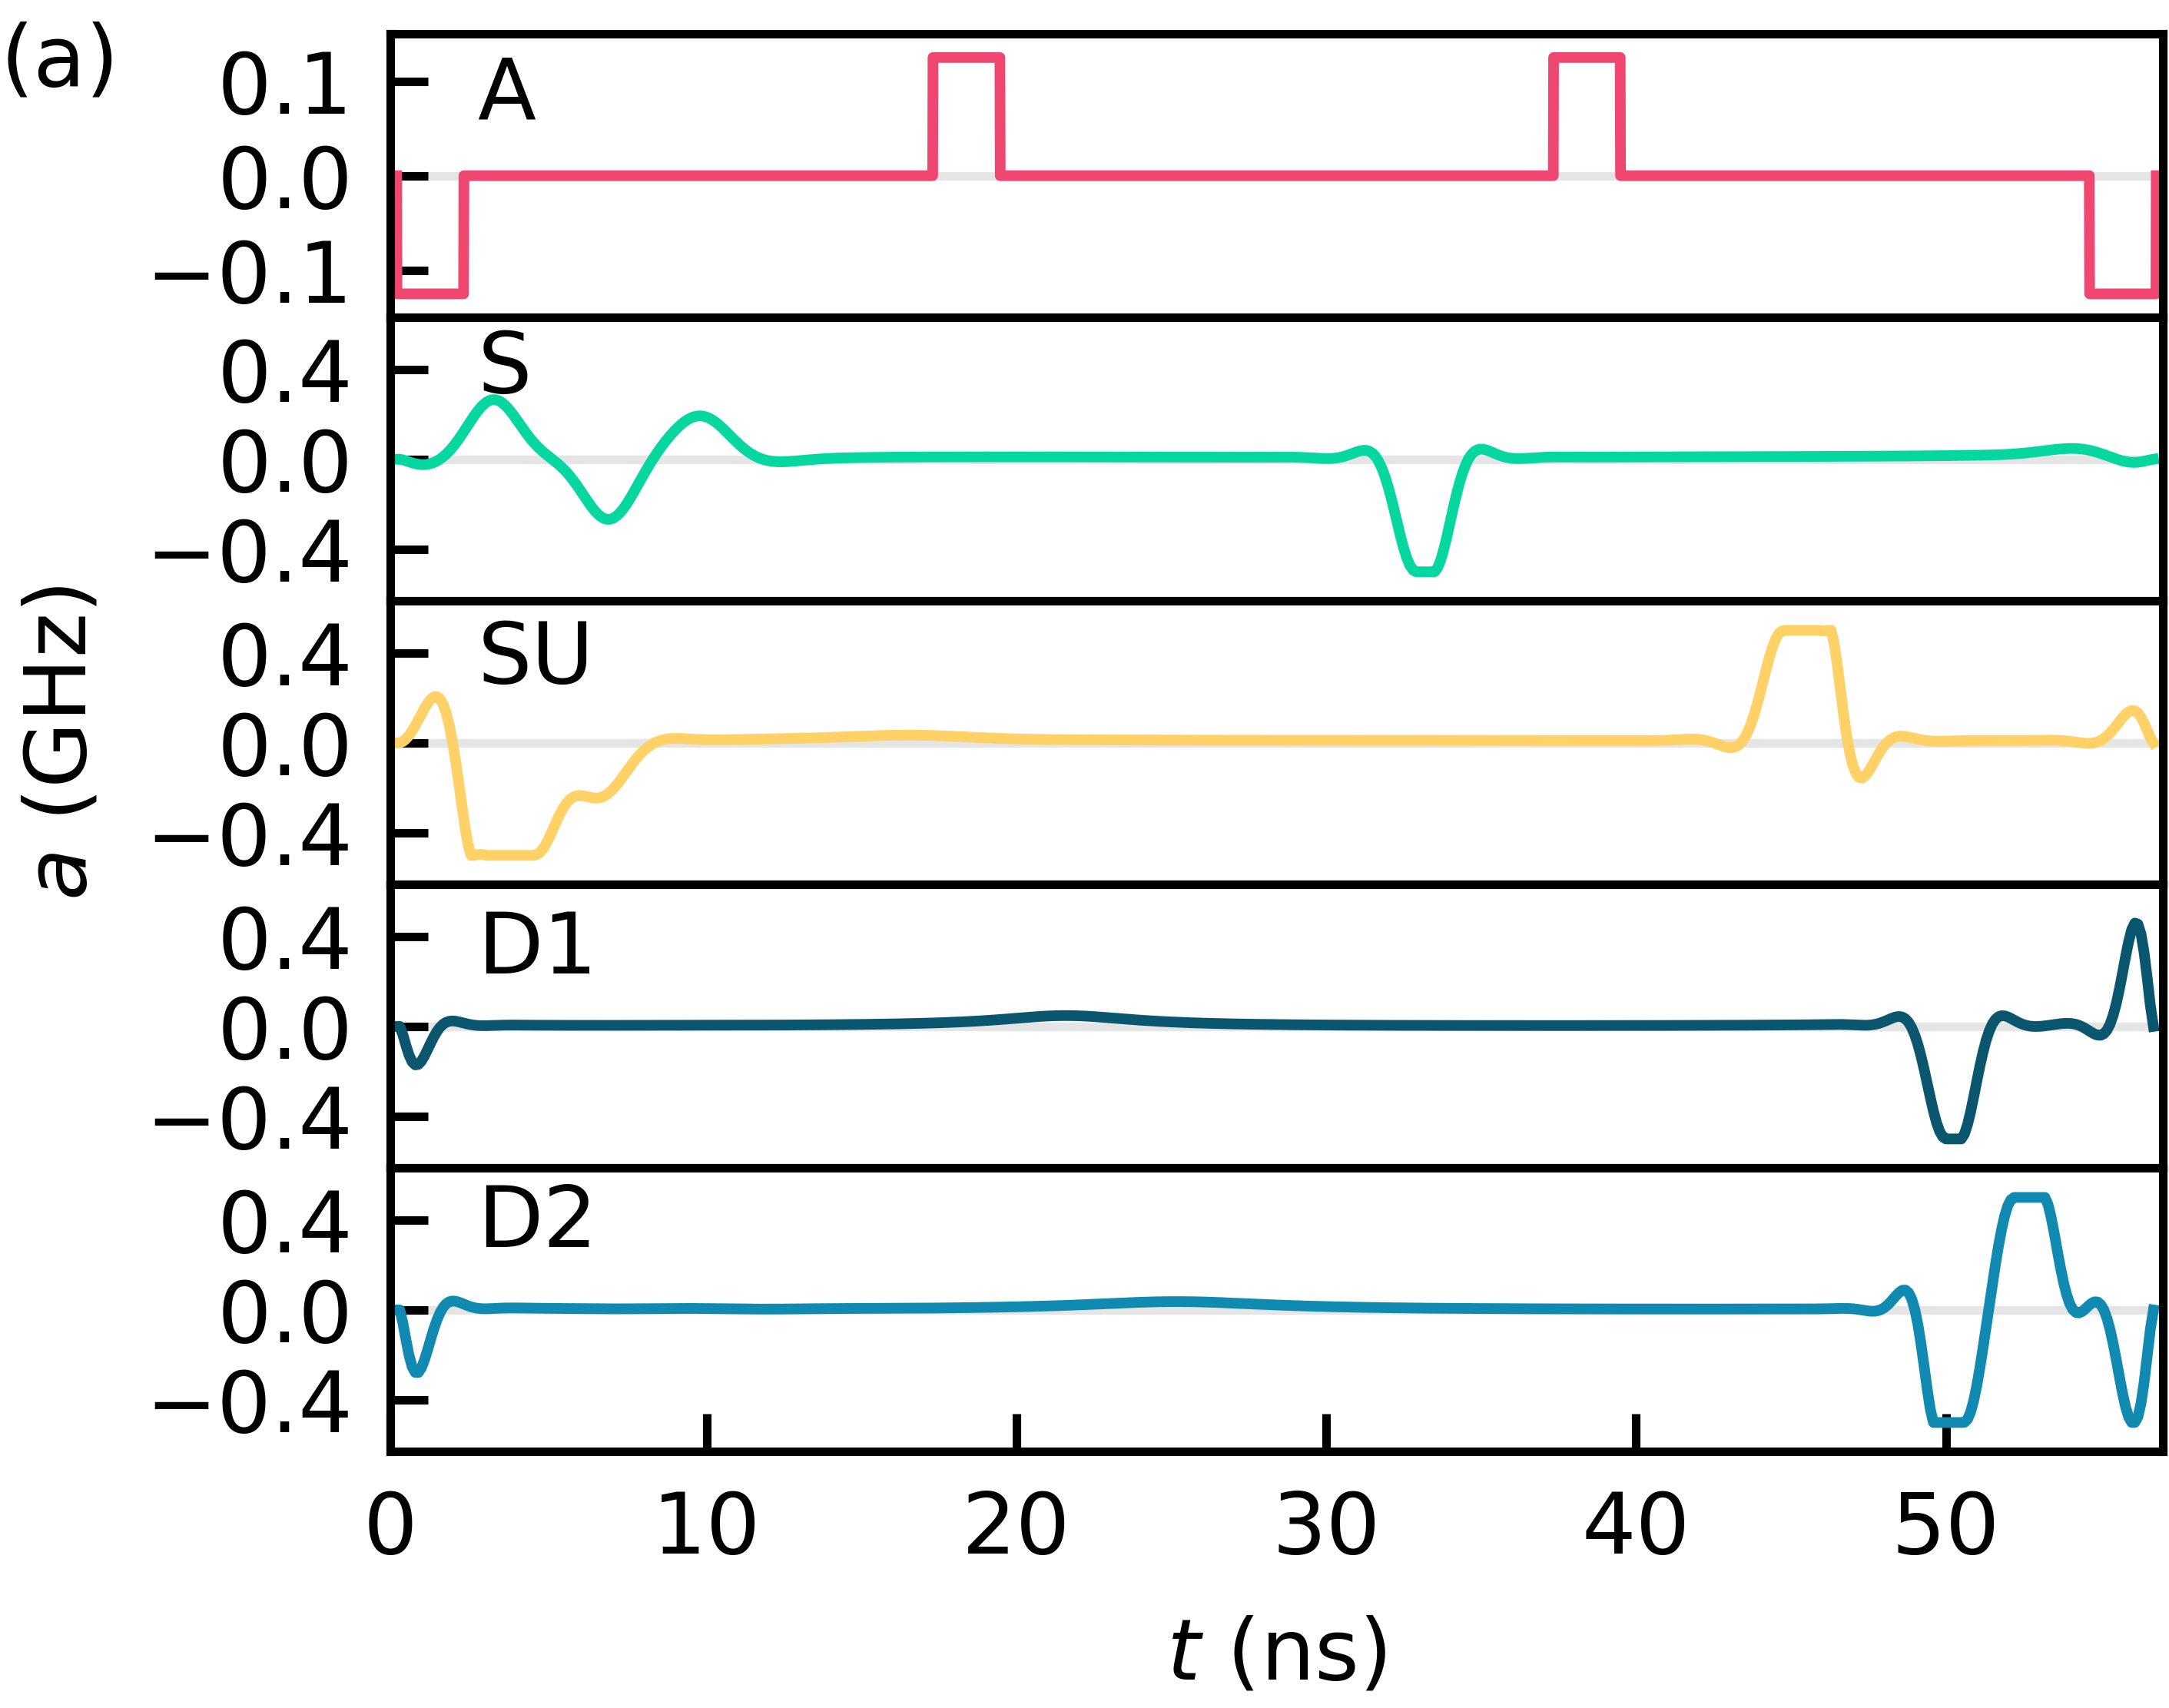
\includegraphics[width=\linewidth]{assets/f3a.png}
    \caption{}
    \label{fig:stochastica}
  \end{subfigure}\hspace{0.05\textwidth}
  \begin{subfigure}{.4\textwidth}
    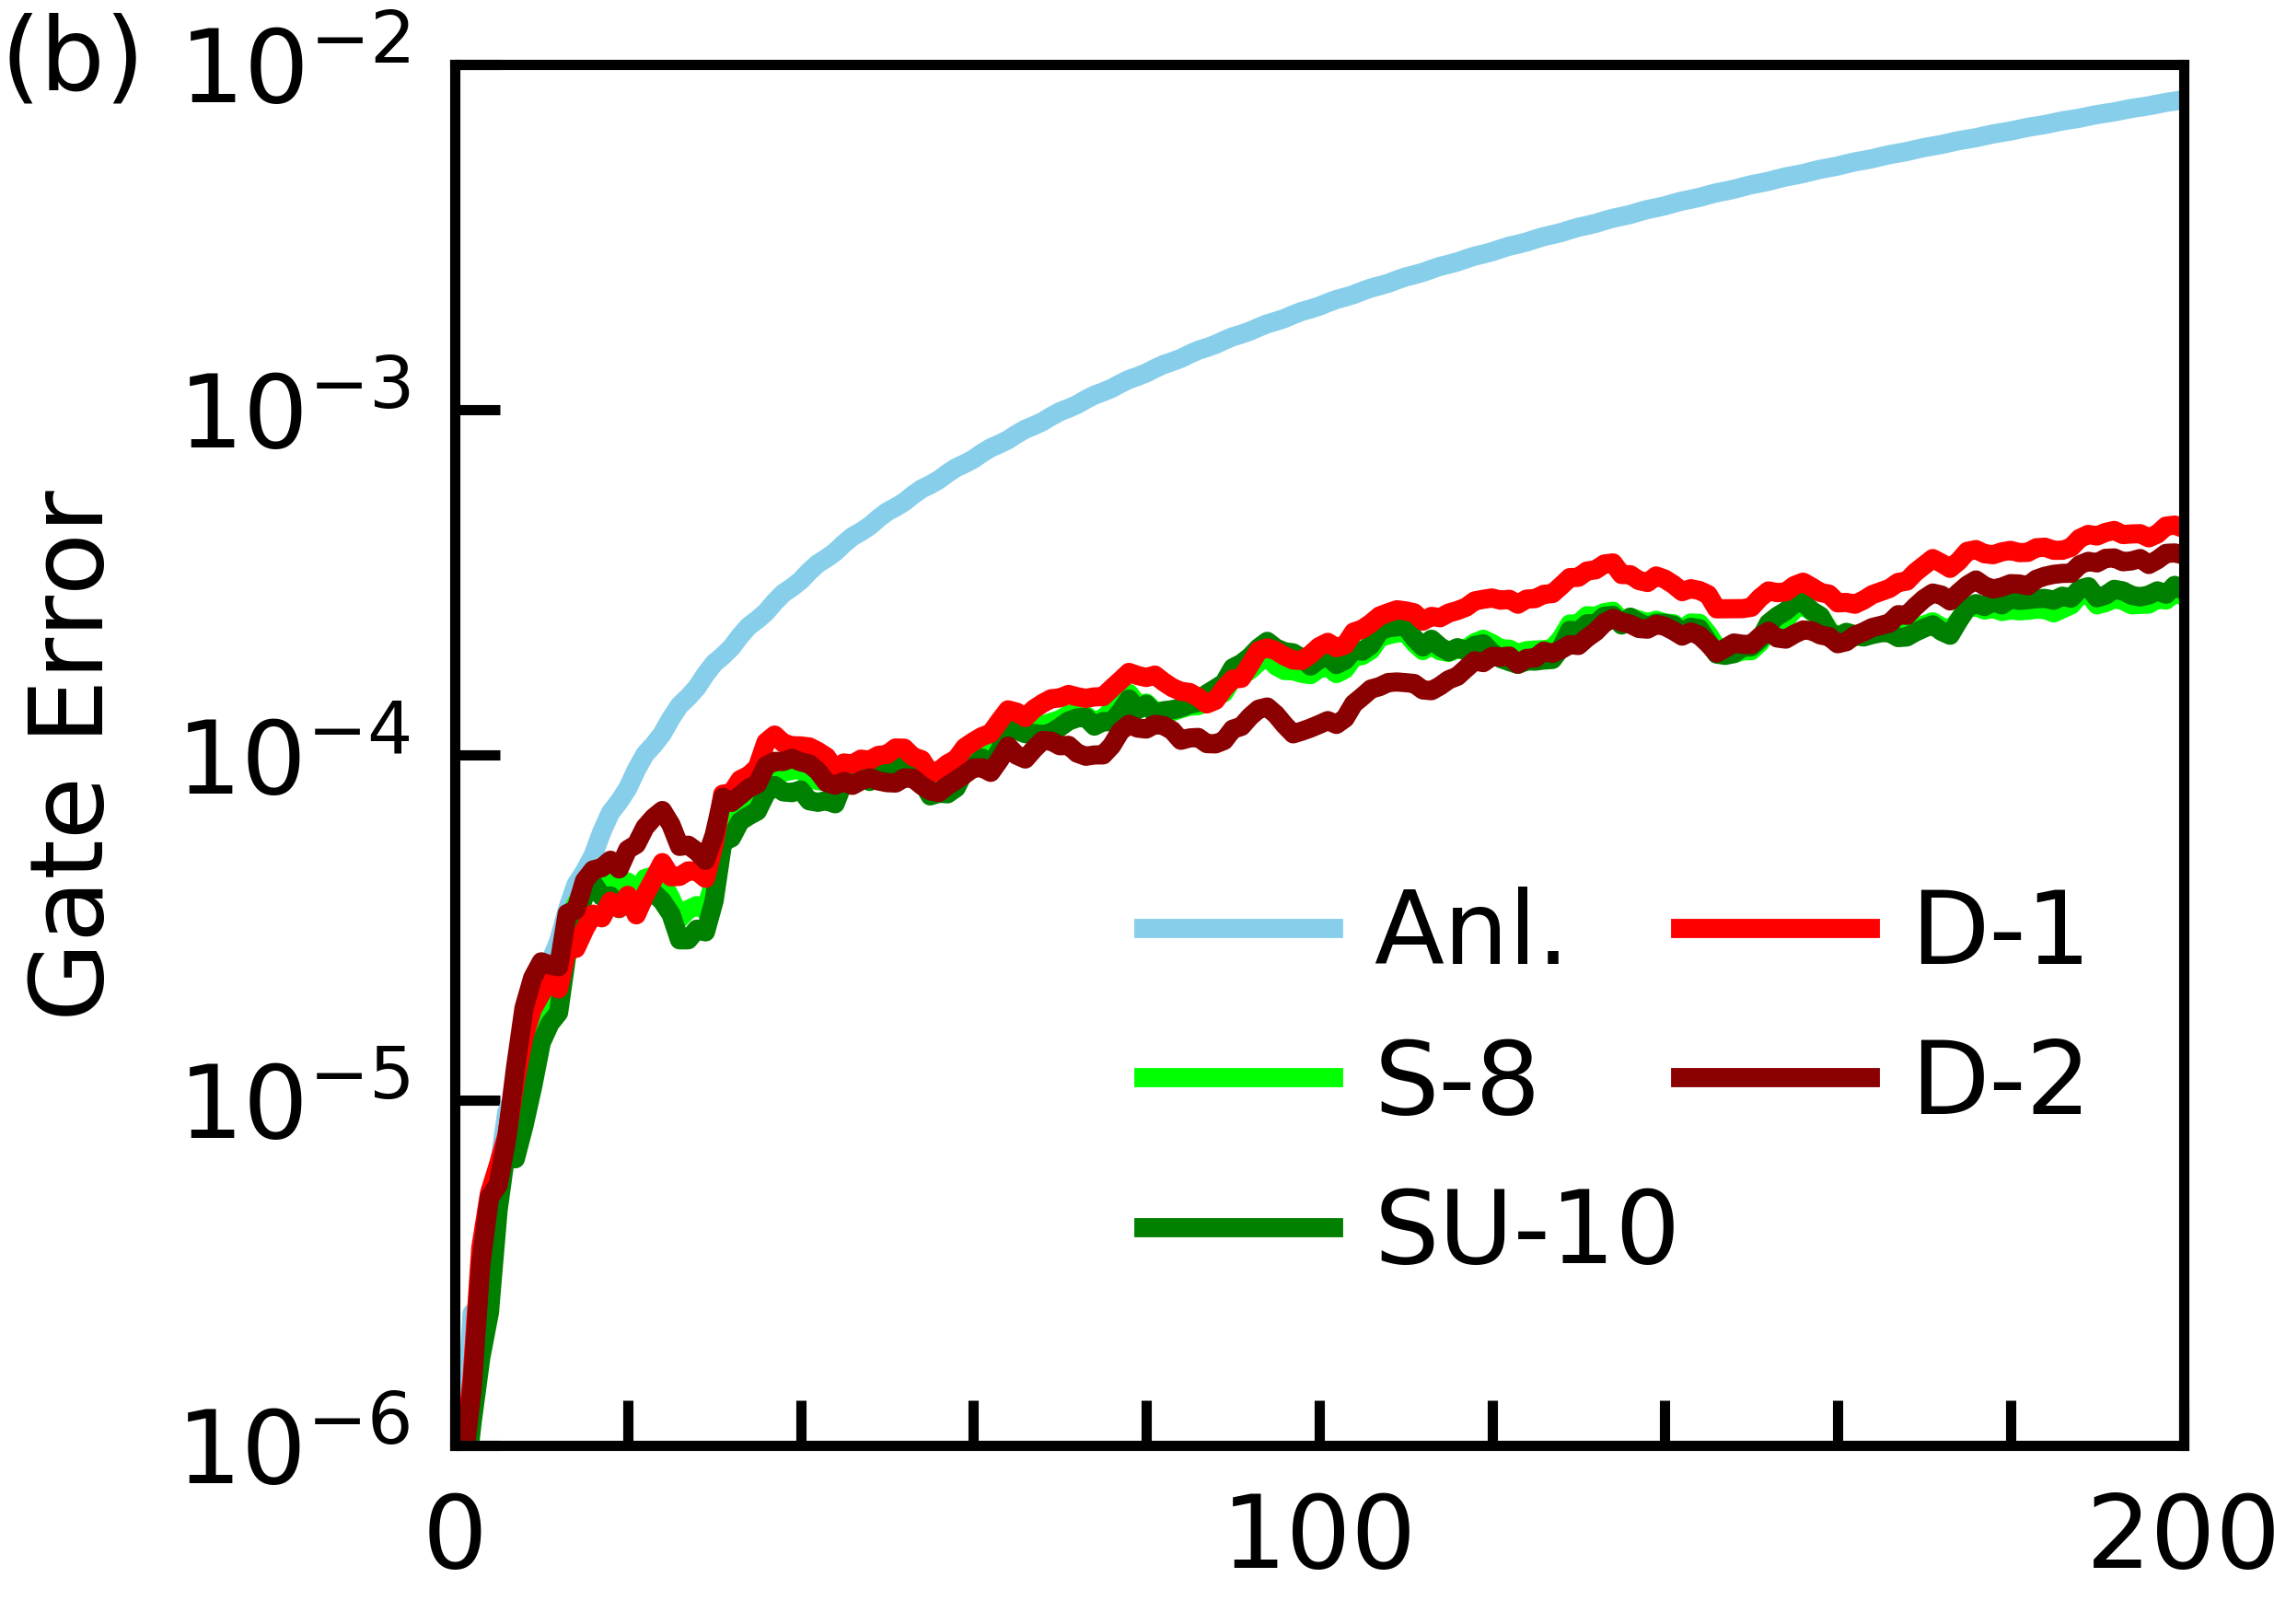
\includegraphics[width=\linewidth]{assets/f3b.png}
        \caption{}
    \label{fig:stochasticb}
  \end{subfigure}
  \caption{
    (a) Flux pulses for $X/2$ gates robust to flux noise
    constructed with the analytic (A),
    sampling (S), unscented sampling (U), and the 1\textsuperscript{st}-
    and 2\textsuperscript{nd}-order derivative methods (D1, D2).
    (b) Cumulative gate error due to 1/$f$ flux noise for
    successive gate applications. The cumulative gate errors for the
    sampling, unscented sampling, and the derivative methods are indistinguishable.
  }
  \label{fig:stochastic}
\end{figure*}

For the sampling method, the gate error at a one-percent qubit frequency detuning
does not decrease substantially over the
range of gate times, and begins to increase above $5 \cdot 10^{-5}$ for gate times
greater than $\sim 50$ns, see Figure \ref{fig:staticb}.
Optimization results for the sampling method reveal that it is typically
able to achieve a high fidelity for
one sample $\ket{\psi^{\pm}}$,
but not the other $\ket{\psi^{\mp}}$, indicating that it is difficult for the optimizer
to make progress on both objectives.
For the unscented sampling method,
the gate error at a one-percent detuning
does not decrease substantially 
over the gate times, but it does reach
a minimum of $\sim 3.9 \cdot 10^{-5}$
near fractions of the Larmor period $2/4f_{q} \sim 36\textrm{ns}$,
$3/4f_{q} \sim 54\textrm{ns}$, $4/4f_{q} \sim 72\textrm{ns}$.

The two derivative methods converge on qualitatively similar flux pulses that
idle near the flux frustration point and use fast triangle movements at the boundaries,
similar to the flux pulse produced by the unscented sampling method.
For both methods, the gate error at a one-percent qubit frequency detuning
decreases super-linearly in the gate time.
For the 1\textsuperscript{st}-order method, the gate error at a one-percent detuning 
reaches $10^{-7}$ at the Larmor period $1 / f_{q} \sim 72$ns,
see Figure \ref{fig:staticc}.
This result mimics the
ability of composite pulses to mitigate parameter uncertainty errors to arbitrary
order with sufficiently many pulses \cite{merrill2014progress}.
It is difficult to choose an appropriate composite pulse
for the problem studied here due to our Hamiltonian and experimental constraints.
We propose comparisons between composite pulses and numerical techniques
for future work.

Furthermore, the ability to perform
$Z$-type gates in any given time is critical
for synchronizing phases in multi-qubit experiments,
where the qubits have distinct
frequencies. Notably, the analytic gate studied here cannot be extended
to gate times other than $1 / 4 f_{q}$. 
We can find gates using the numerical methods at
all gate times above $18$ns, see Figure \ref{fig:staticb}.
These numerical methods offer an effective scheme for synchronizing
multi-qubit experiments.
